%%%%%%%%%%%%%%%%%%%%%%%%%%%%%%%%%%%%%%%%%%%%%%%%%%%%%%%%%%%%%%%%%%%%%%
% VM Slides
% February 15, 2016

\documentclass[aspectratio=169]{beamer}
\usepackage{./styles/Presentation}

\title{Virtual Memory}
\subtitle{A Project for CS854}

\author[N. Chen, S. Pratt, K. Vaidyanathan]{Nick Chen\\Simon Pratt\\%
Krishna Vaidyanathan}

\institute[UW]{University of Waterloo}

\date{\today}

\newcommand{\bi}{\begin{itemize}}
\newcommand{\ei}{\end{itemize}}

\newcommand{\bn}{\begin{enumerate}}
\newcommand{\en}{\end{enumerate}}

%%% BEGIN DOCUMENT
\begin{document}

\frame[plain]{\titlepage}

\begin{frame}{Abstract}
  \begin{columns}[T]
    \begin{column}{0.2\textwidth}
    \end{column}
    \begin{column}{0.6\textwidth}
      In short:
      \bi
      \pause
    \item We propose to study virtual memory!
      \ei
    \end{column}
    \begin{column}{0.2\textwidth}
    \end{column}
  \end{columns}
\end{frame}

\begin{frame}{Proposal}
  \begin{columns}[T]
    \begin{column}{0.2\textwidth}
    \end{column}
    \begin{column}{0.6\textwidth}
      Our proposal has 3 parts:
      \bn
      \pause
    \item {\color<5>{red} Literature Review}
      \pause
    \item Experimental Design
      \pause
    \item Implementation
      \en
    \end{column}
    \begin{column}{0.2\textwidth}
    \end{column}
  \end{columns}
\end{frame}

\begin{frame}{Proposal: Literature Review}
  \begin{columns}[T]
    \begin{column}{0.4\textwidth}
      We wish to investigate the following operating systems:
      \bn
      \pause
    \item Linux
      \pause
    \item NetBSD
      \pause
    \item OpenIndiana\\(Previously Solaris)
      \en
    \end{column}
    \begin{column}{0.6\textwidth}
      \pause
    For each OS, we wish to answer the following questions:
    \bi
    \pause
  \item How is physical memory managed?
    \pause
  \item Are there data structures for physical pages, separate from
    the page tables?
    \pause
  \item How are contiguous regions of memory managed?
    \pause
  \item How is memory freed?
    \pause
    \bi
  \item What happens when the kernel runs out of memory?
    \ei
    \pause
  \item Do they do anything special on Non-Uniform Memory Access
    (NUMA) architectures?
    \ei
    \end{column}
  \end{columns}
\end{frame}

\begin{frame}{Proposal}
  \begin{columns}[T]
    \begin{column}{0.2\textwidth}
    \end{column}
    \begin{column}{0.6\textwidth}
      Our proposal has 3 parts:
      \bn
    \item Literature Review
    \item {\color<2>{red} Experimental Design}
    \item Implementation
      \en
    \end{column}
    \begin{column}{0.2\textwidth}
    \end{column}
  \end{columns}
\end{frame}

\begin{frame}{Proposal: Experimental Design}
  \begin{columns}[T]
    \begin{column}{0.2\textwidth}
    \end{column}
    \begin{column}{0.6\textwidth}
      \bi
      \pause
    \item Make a \emph{testable} hypothesis based on lit. review
      \pause
    \item Design \emph{simple} experiments to test this hypothesis
      \pause
    \item Example:
      \bi
      \pause
    \item Implement data structures from different VMs
      \pause
    \item Test performance
      \ei
      \ei
    \end{column}
    \begin{column}{0.2\textwidth}
    \end{column}
  \end{columns}
\end{frame}

\begin{frame}{Proposal}
  \begin{columns}[T]
    \begin{column}{0.2\textwidth}
    \end{column}
    \begin{column}{0.6\textwidth}
      Our proposal has 3 parts:
      \bn
    \item Literature Review
    \item Experimental Design
    \item {\color<2>{red} Implementation}
      \en
    \end{column}
    \begin{column}{0.2\textwidth}
    \end{column}
  \end{columns}
\end{frame}

\begin{frame}{Proposal: Implementation}
  \begin{columns}[T]
    \begin{column}{0.2\textwidth}
    \end{column}
    \begin{column}{0.6\textwidth}
      \bi
      \pause
    \item Optional
      \pause
    \item Implement a memory management system for KOS
      \pause
    \item Use findings from:
      \bi
      \pause
    \item Lit review
      \pause
    \item Experiments
      \ei
      \ei
    \end{column}
    \begin{column}{0.2\textwidth}
    \end{column}
  \end{columns}
\end{frame}

\begin{frame}{High-level design}
  \begin{columns}[T]
    \begin{column}{0.2\textwidth}
    \end{column}
    \begin{column}{0.6\textwidth}
      We now understand the VM design at a high-level:
      \bi
      \pause
    \item Linux
      \pause
    \item NetBSD
      \pause
    \item OpenIndiana
      \ei
    \end{column}
    \begin{column}{0.2\textwidth}
    \end{column}
  \end{columns}
\end{frame}

\begin{frame}{High-level: Linux}
  \begin{columns}[T]
    \begin{column}{0.4\textwidth}
      \bi
    \item vm\_area\_struct
      \ei
      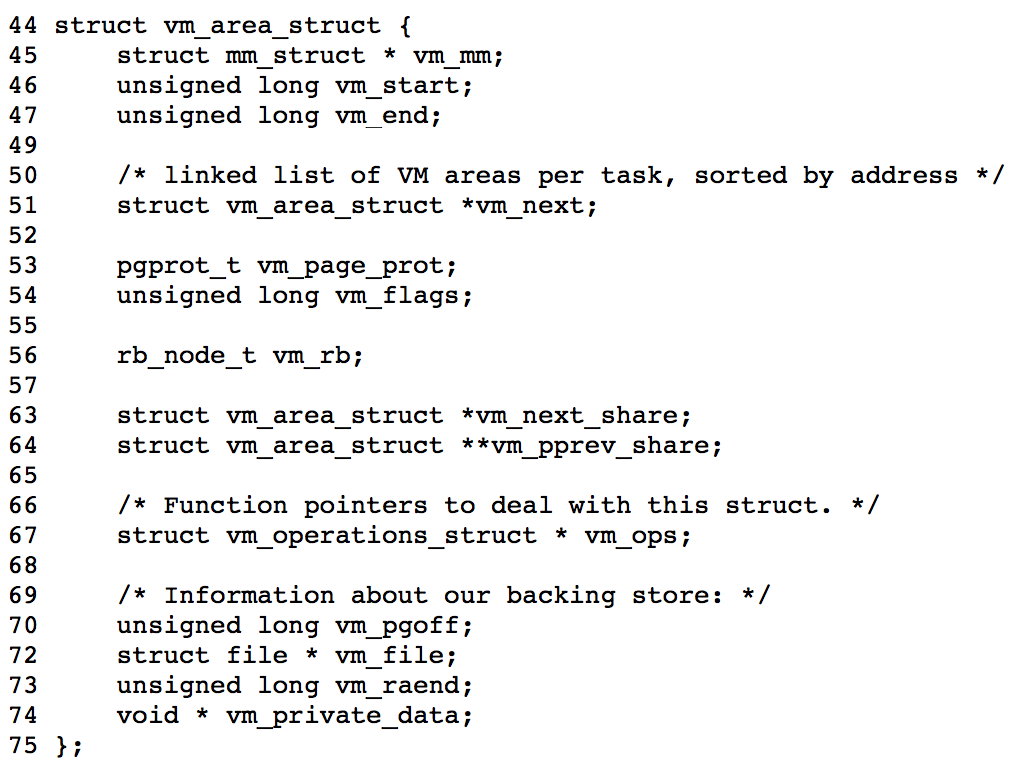
\includegraphics[scale=0.35]{./figures/linux3.png}
    \end{column}
    \begin{column}{0.6\textwidth}
      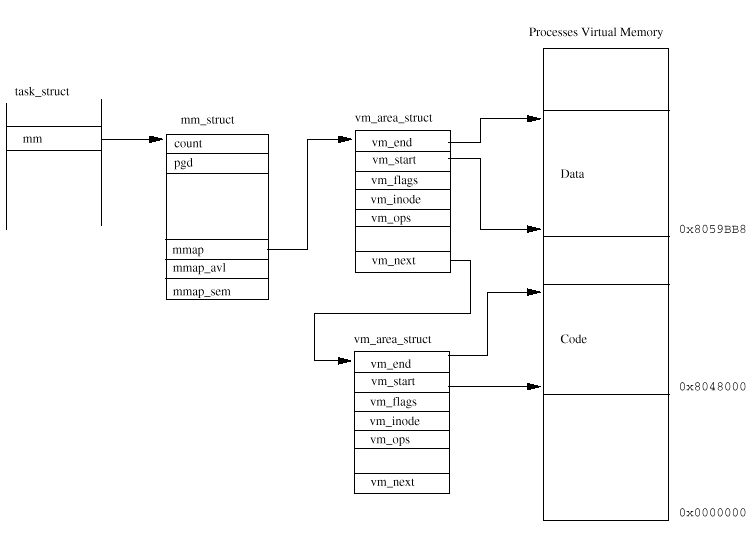
\includegraphics[scale=0.35]{./figures/linux1.png}
    \end{column}
  \end{columns}
\end{frame}

\begin{frame}{High-level: NetBSD}
  \begin{columns}[T]
    \begin{column}{0.6\textwidth}
      \includegraphics<5->[scale=0.35]{./figures/uvm.png}
    \end{column}
    \begin{column}{0.4\textwidth}
      \bi
    \item Based on 386BSD, 4.4BSD-Lite
      \pause
    \item Rewritten in 1998 by Chuck Cranor
      \bi
      \pause
    \item UVM (Unified(?) VM)
      \pause
    \item 13 page Usenix paper
      \pause
    \item 270 page PhD dissertation
      \ei
      \pause
    \item Slightly modified in 2001 by Chuck Silvers
      \bi
      \pause
    \item UBC (Unified Buffer Cache)
      \pause
    \item 5 page Usenix paper
      \ei
      \pause
    \item Minor modifications since then
      \ei
    \end{column}
  \end{columns}
\end{frame}

\begin{frame}{High-level: OpenIndiana}
    \begin{enumerate}
        \item Open source fork of OpenSolaris after Oracle take over
        \item Stewarded by the Illumos Foundation
    \end{enumerate}
\end{frame}

\begin{frame}{Virtual memory management unit}
    \begin{enumerate}
        \item Solaris kernel breaks up virtual address space into mappings for
            each type of memory (eg., heap, stack)
        \item Hardware MMU maps pages to physical memory using platform-specific
            translation tables
        \item Memory management to manage pages is basically swapping and demand
            paging
    \end{enumerate}
\end{frame}

\begin{frame}{Solaris 10 Virtual to Physical Memory Management}
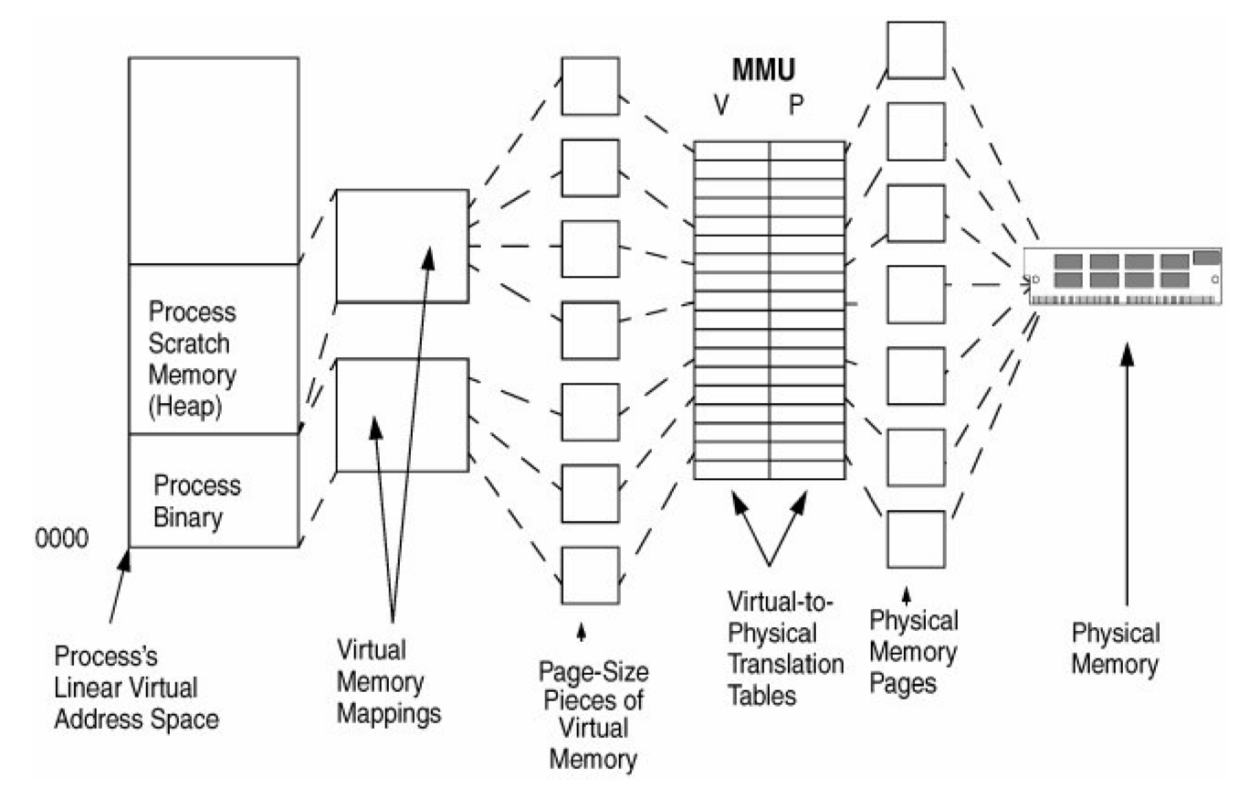
\includegraphics[scale=0.20]{./figures/openindiana_mmu.jpg}
\end{frame}

\begin{frame}{Solaris 10 page table structure}
    \begin{columns}[T]
        \begin{column}{0.6\textwidth}
            \includegraphics<1->[scale=0.15]{./figures/page_structure.png}
        \end{column}
        \begin{column}{0.4\textwidth}
            \bi
                \item Page table structure different from x86 hardware page table
                    structure
            \ei
        \end{column}
    \end{columns}
\end{frame}

\begin{frame}{Differences}
  \begin{columns}[T]
    \begin{column}{0.2\textwidth}
    \end{column}
    \begin{column}{0.6\textwidth}
      We have found some significant differences so far:
      \bi
      \pause
    \item What happens when the kernel runs out of memory?
      \pause
    \item What are the copy-on-write mechanisms?
      \ei
    \end{column}
    \begin{column}{0.2\textwidth}
    \end{column}
  \end{columns}
\end{frame}

\begin{frame}{What happens when the kernel runs out of memory?}
  \begin{columns}[T]
    \begin{column}{0.3\textwidth}
      Linux:
      \bi
    \item Start killing processes
      \ei
      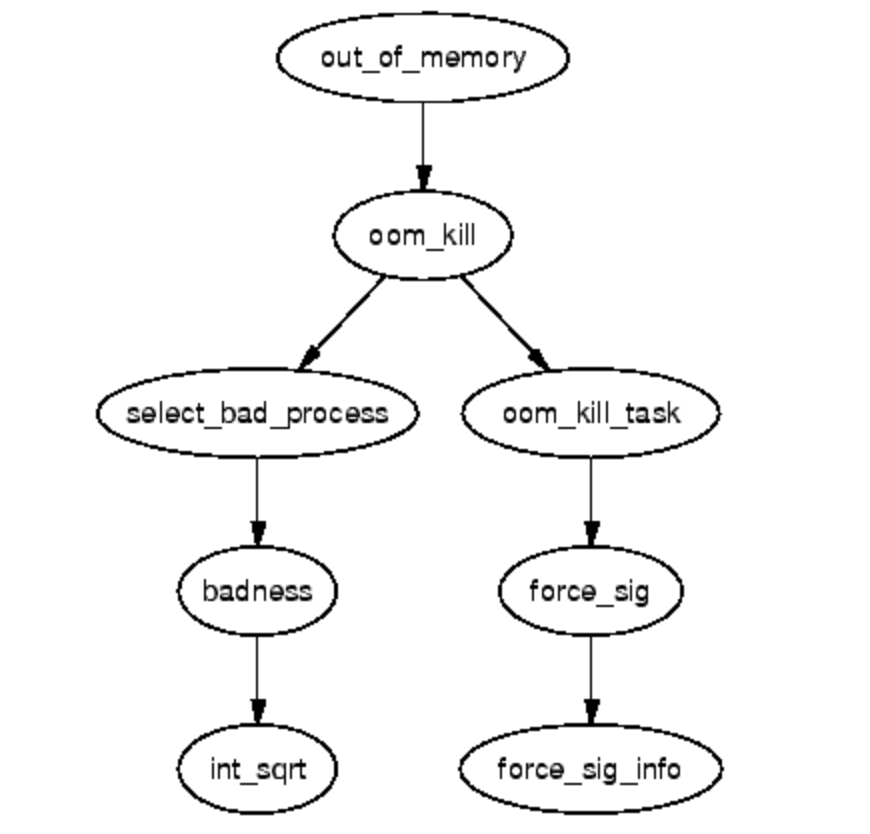
\includegraphics[scale=0.35]{./figures/linux4.png}
    \end{column}
    \pause
    \begin{column}{0.4\textwidth}
      NetBSD:
      \bi
    \item Panic!
      \ei
    \end{column}
    \pause
    \begin{column}{0.3\textwidth}
      OpenIndiana:
      \bi
    \item Periodically checks kernel space, and "snaps" data to user space if
        kernel space is low
    \item If kernel runs out of memory, crashes as far as I can tell
      \ei
    \end{column}
  \end{columns}
\end{frame}

\begin{frame}{What are the copy-on-write mechanisms?}
  \begin{columns}[T]
    \begin{column}{0.3\textwidth}
      Linux:
      \bi
    \item Page-based copy
      \ei
    \end{column}
    \pause
    \begin{column}{0.3\textwidth}
      OpenIndiana:
      \bi
    \item Anonymous maps
      \ei
    \end{column}
    \pause
    \begin{column}{0.4\textwidth}
      NetBSD:
      \bi
    \item Copied SunOS/Solaris
      \ei
    \end{column}
  \end{columns}
\end{frame}

\begin{frame}{Summary}
  \begin{columns}[T]
    \begin{column}{0.2\textwidth}
    \end{column}
    \begin{column}{0.6\textwidth}
      \bn
    \item Literature Review
      \bi
    \item High-level design
    \item Differences
      \ei
    \item Experimental Design
    \item Implementation
      \en
    \end{column}
    \begin{column}{0.2\textwidth}
    \end{column}
  \end{columns}
\end{frame}

\begin{frame}[noframenumbering]{References}
  \small
  \bi
\item UVM dissertation:\\
  \url{http://vorpal.math.drexel.edu/course/opsys2/uvm-project/uvm.pdf}
\item UVM paper:\\
  {\footnotesize\url{https://www.usenix.org/legacy/event/usenix99/full_papers/cranor/cranor.pdf}}
\item UBC paper:\\
  \url{https://www.usenix.org/legacy/publications/library/proceedings/usenix2000/freenix/silvers.html}
\item \textsl{Understanding the Linux Virtual Memory Manager}\\
  \url{https://www.kernel.org/doc/gorman/html/understand/index.html}
\item McDougall, Richard, and Jim Mauro. Solaris internals: Solaris 10 and OpenSolaris kernel architecture. Pearson Education, 2006.
  \ei
\end{frame}

\begin{frame}[noframenumbering]{Attribution}
  \bi
\item NetBSD data structure diagram from:\\
  {\tiny\url{http://usenix.org/legacy/publications/library/proceedings/usenix99/full_papers/cranor/cranor_html/index.html}}
\item Linux vm\_area\_struct source from:\\
  \url{???}
\item Linux data structures diagram from:\\
  \url{???}
\item Linux OOM diagram from:\\
  \url{???}
\item Solaris VM diagram:\\McDougall, Richard, and Jim Mauro. Solaris internals: Solaris 10 and
    OpenSolaris kernel architecture. Pearson Education, 2006.
  \ei
\end{frame}

\begin{frame}[noframenumbering]{License}
  \bi
\item These slides are distributed under the creative commons
  Attribution-ShareAlike 4.0 International (CC BY-SA 4.0).
\item See http://creativecommons.org/licenses/by-sa/4.0/ for details.
  \ei
\end{frame}

\end{document}
